\documentclass{llncs}
\usepackage{graphicx}
\usepackage{subcaption}
\captionsetup{compatibility=false}
\usepackage{url}
\usepackage{amsmath}
\usepackage{amssymb}
\usepackage[]{algorithm2e}
\usepackage{tabularx}
\DeclareMathOperator*{\argmax}{arg\,max}

% --- TITLE AND AUTHOR INFORMATION
\title{Heterogeneous Multi-Agent Deep Reinforcement Learning for Traffic Lights Control}
\author{Jeancarlo Arguello Calvo, Ivana Dusparic}
\institute{School of Computer Science and Statistics, University of Dublin, Trinity College \\
\email{arguellj@tcd.ie, ivana.dusparic@scss.tcd.ie} }
% --- END OF PREAMBLE 

% --- START DOCUMENT
\begin{document}
\maketitle

\begin{abstract}
The most promising technique used in urban traffic control (UTC) has been Reinforcement Learning (RL) due to its capacity to learn the dynamics of complex problems. The main problem of this approach is the curse of dimensionality that arises from the exponential growth of the state and action spaces because of the number of intersections.
	
	Deep Reinforcement Learning (DRL) enhances hugely the performance of RL. DRL has proved to work very well for UTC in single agent environments. Nonetheless, when the problem scales up to multiple intersections the need for coordination becomes too complex, and as a result, the latest studies take advantage of the similarity of agents to train them as one. However, the usage of homogeneous junctions is not a real world scenario where a city has different layouts of intersections.
	
	This study proposes the usage of Independent Deep Q-Network (IDQN) to train heterogeneous multi-agents to deal with both the curse of dimensionality and the need for collaboration. The former is handled by using Deep Q-Networks. The latter is managed with IDQN, which trains simultaneously and separately each agent allowing us to support heterogeneous agents. Unfortunately, this technique can lead to convergence problems because one agent's learning makes the environment appear non-stationary to other agents, and this problem conflicts with experience replay memory on which DQN relies. We address this issue by conditioning each agent's value function on a fingerprint that disambiguates the age of the data sampled from the replay memory.
\end{abstract}

\section{Introduction}

This research addresses heterogeneous multi-agents for  urban traffic control (UTC) systems as the first study applying Deep Reinforcement Leaning (DRL) in a heterogeneous network layout which is a reflection of the cities in the real world. It proposes the usage of DRL to deal with the curse of dimensionality that suffers RL approaches by using Neural Networks. It also uses Indepedent Q-Learning (IQL), where each agent learns independently and simultaneously its own policy, treating other agents as part of the environment. However, the environment becomes nonstationary from the point of view of each agent, as it involves the interaction with other agents who are themselves learning at the same time, ruling out any convergence guarantees. The technique used for this problem is Deep Q-Networks which relies in a component so called experience replay memory in order to stabilize and improve the learning. However, this memory is incompatible with non-stationary environments. In order to combine the experience replay memory and IQL, we used a technique of fingerprinting which stabilizes the memory against the non-stationarity. This fingerprint disambiguates the age of the data sampled from the replay memory. We evaluate the usage of IQL with Deep Q-Networks in a multi-agent setting by using a simulation of an urban traffic control system.


\section{Background and Related Work}

\subsection{Reinforcement Learning}

Reinforcement learning (RL) is about learning optimal actions from specific situations where the agent has to discover which actions maximize a reward signal by exploring them in a trial-and-error basis. These actions may affect future situations and subsequent reward signals \cite{RichardS.SuttonandAndrewG.Barto2018}.

In RL an agent interacts with the environment. On each time step t, the agent perceives an state \textit{s$_{t}$} in state space \textit{S} from where it selects an action \textit{a$_{t}$} in the action space \textit{A} by following a policy \textit{$\pi$}. The agent receives a reward \textit{r$_{t}$} when it transitions to the state \textit{s$_{t+1}$} according to the environment dynamics, the reward function  \textit{R(s$_{t}$, a$_{t}$, s$_{t+1}$)} and the transition function \textit{T(s$_{t}$, a$_{t}$, s$_{t+1}$)}. In order to converge the algorithm faster, a discount factor $\gamma$ $\in$ [0, 1] is applied to the total amount of reward.

RL can be either model-based or model-free (where the transition and the reward functions are unknown). The most common model-free technique is Q-Learning, where RL agents learn Q-values which are functions of state-action pair that returns a real value: \textit{Q: S} x \textit{A $\rightarrow$ $\mathbb{R}$}. Thus, the policy is represented as:

\begin{equation}
\pi(s) = \argmax_{a \in A} Q(s, a)
\end{equation}

where the Q-value can be learned by using Q-learning updates \cite{Watkins1992}:

\begin{equation}
Q(s, a) = (1 - \alpha)Q(s, a) + \alpha[R(s, a) + \max_{a \in A}Q(s', a')]
\end{equation}

where 0 $<$ $\alpha$ $\leq$ 1 is a learning rate.


\subsection{Deep Reinforcement Learning}

The curse of dimensionality given by large state and action spaces make unfeasible to learn Q value estimates for each state and action pair independently as in normal tabular Q-Learning. Therefore, DRL models the components of RL with deep neural networks. The following subsections describe the methods used during the proposed research to implement the Deep Reinforcement Learning in Traffic Light problem.

\subsubsection{Deep Q Networks}

\cite{Mnih2015} proposed Deep Q-Networks (DQN) as a technique to combine Q-Learning with deep neural networks. RL is known to be unstable or even to diverge when a non-linear function approximator such as a neural network is used to represent the Q value. DQN addresses these instabilities by using two insights, experience replay and target network.
	
	DQN parameterizes an approximate value function Q(s, a; $\theta_{i}$) using Convolutional Neural Networks, where $\theta_{i}$ are the weights of the network at iteration i. The experience replay stores the agent's experiences e$_{t}$ = (s$_{t}$, a$_{t}$, r$_{t}$, s$_{t+1}$) at each time step t in a dataset D$_{t}$ = {e$_{1}$,…,e$_{t}$} pooled over many episodes into a replay memory. Then, mini batches of experience drawn uniformly at random from the dataset (s, a, r, s) $\sim$ U(D) are applied as Q-updates during the training. The Q-learning update at iteration i follows the loss function:
	
\begin{equation}
L_{i}(\theta_{i}) = \ E_{(s,a,r,s) \sim U(D)} \left[ \left(r + \gamma \max_{a'}Q\left(s',a';\theta_{i}^{-}\right) - Q\left(s,a;\theta_{i}\right)\right)^{2} \right]
\end{equation}

where $\theta_{i}$ are the parameters of the Q-network at iteration i and $\theta_{i}^{-}$ are the target network parameters. The target network parameters are only updated with the Q-network parameters every C steps and are held fixed between individual updates.

\subsubsection{Double DQN}

	The max operator in standard Q-learning and DQN uses the same values both to select and to evaluate an action. It is known the this maximization sometimes produces to learn unrealistically high action values which tends to prefer overestimated values over underestimated values, resulting in overoptimistic value estimations. To prevent this, Double Q-learning decouples the selection and the evaluation \cite{Hasselt2010}.
	
	For DQN architectures is not desired to fully decoupled the target  as in \cite{Hasselt2010} because the target network provides a intuitive option for the second value function, without having to include extra networks. For that reason, \cite{Hasselt:2016:DRL:3016100.3016191} propose to evaluate the greedy policy according to the online network, but using the target network to estimate its value given as result the Double DQN (DDQN) algorithm:
	
\begin{equation}
Y_{t}^{DDQN} = R_{t+1} + \gamma Q(s_{t+1}, \argmax_{a} Q(s_{t+1}, a;\theta_{t});\theta_{i}^{-})
\end{equation}

\subsubsection{Prioritized Experience Replay}

\cite{SchaulQAS15} presented prioritized experience replay which detaches agents from considering transitions with the same frequency that they are experienced. Prioritized replay samples more frequently transitions from which there is a high expected learning progress. as measured by the magnitude of their temporal-difference (TD) error. It samples transitions with probability p$_{t}$ relative to the last encountered absolute TD error:
	
\begin{equation}
p_{t} \propto \left|\left(R_{t+1} + \gamma_{t+1} \max_{a'}Q\left(s',a';\theta_{i}^{-}\right) - Q\left(s,a;\theta_{i}\right)\right)\right|^{\omega}
\end{equation}

Where $\omega$ is a hyper-parameter that determines the pattern of the distribution. New transitions are pushed into the replay buffer memory with maximum priority, providing a bias towards recent transitions.

\subsubsection{Dueling Network}\label{duelingNet}

Dueling Network is a technique proposed by \cite{Wang2016} which computes separately the value V(s) and advantage A(s, a) functions that are represented by a duelling architecture that consists of two streams where each stream represents one of these functions. These two streams are combined by an convolutional layer to produce an estimate of the state-action value Q(s, a). The dueling network automatically produces separate estimates of the state value and advantage functions without supervision. Besides that, it can learn which states are valuable, without having to explore the consequence of each action for each state. Dueling network is defined with the equation:

\begin{equation} \label{eq:dueling eq}
Q(s,a;\theta,\alpha,\beta) = V(s;\theta,\beta) + \left( A\left(s,a;\theta,\alpha \right) - \frac{1}{|\mathcal{A}|} \displaystyle\sum_{a'} A\left(s,a;\theta,\alpha \right) \right) 
\end{equation}
	
\subsection{Multi-Agent Reinforcement Learning} \label{sec:MARL}

Consider a cooperative multi-agent environment where \textit{n} agents identified by a $\epsilon$ A $\equiv$ $\{$1,..., n$\}$ participate in a stochastic game G, denoted by a tuple $<$S, U, P, r, Z, O, n, $\gamma>$. The environment consists of states s$_{t}$ $\epsilon$ S, where at every time step t, each agent takes an action \textit{u$^{a}_{t}$} $\epsilon$ U, forming a joint action \textbf{u$_{t}$} $\epsilon$ \textbf{U} $\equiv$ U$^{n}$.
The transition probabilities are defined by P(s$_{t+1}$ $|$ s$_{t}$, u$_{t}$) : S x U x S $\rightarrow$ [0, 1]. A global reward function r(s$_{t}$, u$_{t}$) : S x U $\rightarrow$ $\mathbb{R}$ is shared between all the agents.

Each agent's observations z $\epsilon$ Z follows an observation function O(s$_{t}$, a) : S x A $\rightarrow$ Z. Each agent \textit{a} conditions its behaviour on its own action-observation history $\tau_{a}$ $\epsilon$ T $\equiv$ (Z x U)*, according to its policy $\pi_{a}$(u$_{a}$ $|$ $\tau_{a}$) : T x U $\rightarrow$ [0, 1]. After each transition, the action u$_{t}^{a}$ and new observation O(s$_{t}$, a) are added to $\tau_{a}$, forming $\tau_{a}^{'}$. Let the joint quantities over agents be in bold, and the joint quantities over agents other than \textit{a} with the subscript \textit{-a}, so that, e.g., \emph{u} = [u$_{t}^{t}$, \textbf{u}$_{-a}$].

\subsubsection{Independent DQN}

Independent DQN (IDQN) is an extension of Independent Q-Learning\cite{Tan1993} with DQN for cooperative multi-agent environment, where each agent \textit{a} observes the partial state s$_{t}^{a}$, selects an individual action \textit{u$_{t}^{a}$}, and receives a team reward, r$_{t}$ shared among all agents. \cite{Tampuu2015} combines DQN with independent Q-learning, where each agent \textit{a} independently and simultaneously learns its own Q-function \textit{Q$^{a}(s, u^{a};\theta^{a}_{i})$} \cite{DBLP:journals/corr/FoersterAFW16a}. Since our setting is partially observable, IDQN can be implemented by having each agent conditioned on its action-observation history, i.e., Q$_{a}$($\tau_{a}$, u$_{a}$). In DRL, this can be implemented by given to each agent a DQN on its own observations and actions.

As mentioned before, a key component of DQN is the experience replay memory.  Unfortunately, the combination of experience replay with IQL appears to be problematic because the non-stationarity introduced by IQL which provokes that the dynamics that generated the data in the agent's experience replay memory no longer indicate the current dynamics in which the agent is learning.

A fingerprint technique was introduced in \cite{Foerster2017}, which states that the disadvantage of IQL is that it ignores the changing over time of the other agents' policies because it perceives the other agents as part of the environment, which causes non-stationarity on its own Q-function. Hence, the Q-function might be made stationary if it conditioned on the other agents' policies.

Based on the results of the study, a fingerprint must be correlated with the true value of state-action pairs given the other agents' policies. It should gradually change over training time in order to allow the model to generalise across experiences in which the other agents execute policies as they learn.

\subsection{Related Work}

Prior to RDL, several RL approaches for heterogenous multi-agent UTC environments were done as in \cite{Dusparic2016,Chu2017,Tahifa2015,El-Tantawy2012}. However, the techniques used cannot be extended to DRL. Recent works started to explore DRL solutions for UTC in single agent scenarios to deal with the curse of dimensionality as in \cite{Li2016,Mousavi2017,Gao2017,Liang2018}. These studies started to represent the state as snapshots of the intersection in order to use Convolutional Neural Networks. The variables obtained from the images are position and speed of vehicles, however those are processed and expressed differently on each study.

The DNNs architecture are getting more complex over the years. First approaches only considered a simple CNN, but later on the new techniques were aggregated to improve the stability and performance of the training such as DDQN, Dueling Networks and Prioritized Experience Replay. All these single agent approaches obtained good results. Because of that, they were extended to multi-agent scenarios as in \cite{Belletti2018,VanDerPol2016,Liu2017CooperativeDR}. \cite{Belletti2018} used DRL for controlling the metering of highway on-ramps modelling the problem as discretized non-linear partial differential equations in a robust and non-parametric manner. \cite{VanDerPol2016,Liu2017CooperativeDR} implemented solutions for homogeneous multi-agent by taking advantage of the similarity in order to train only one Neural Network which can be used for all agents indistinctly. \cite{VanDerPol2016} used transfer planning and max-plus algorithm. While, \cite{Liu2017CooperativeDR} used a IQL variation where only one agent is trained at each training episode, and the others react based on their previously learned policies. After an amount of iterations, the latest agent's policy is distributed to the other agents, and the training agent is changed to another one to start a new training cycle. 

\section{Design}

\subsection{State Representation}\label{sec:stateRep}

	The state is a image-like representation of the current state of the simulator environment (Figure \ref{fig:simSt}), similar to the concept used in \cite{Mnih2015}. The state consists of two matrices of 64x64: (1) a binary matrix \textit{P} for vehicle positions (Figure \ref{fig:matrixP}), and (2) a matrix \textit{S} for vehicle speeds (Figure \ref{fig:matrixS}). These matrices have been used in previous works such as \cite{Gao2017,Liang2018,Liu2017CooperativeDR,VanDerPol2016}. 
	
\begin{figure}
    \centering
    \begin{subfigure}[b]{0.25\textwidth}
        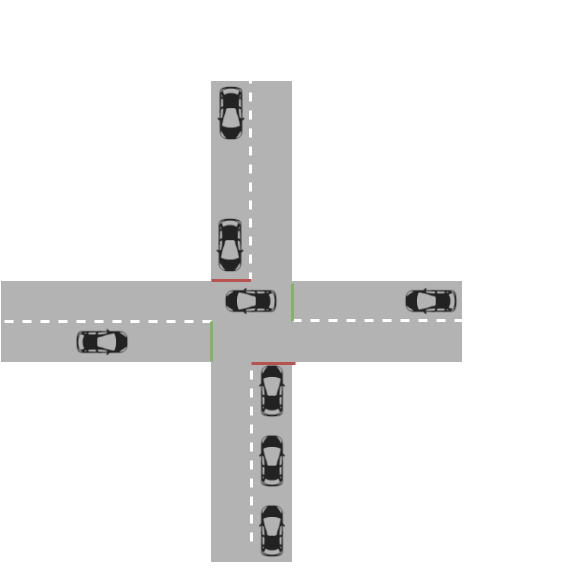
\includegraphics[width=\textwidth]{images/intersection.png}
        \caption{Simulation Environment State}
        \label{fig:simSt}
    \end{subfigure}
    \begin{subfigure}[b]{0.25\textwidth}
	    \small
		$ \begin{bmatrix}
		\centering
		0 & 0 & 0 & 1 & 0 & 0 & 0 & 0 \\
		0 & 0 & 0 & 0 & 0 & 0 & 0 & 0 \\
		0 & 0 & 0 & 1 & 0 & 0 & 0 & 0 \\
		0 & 0 & 0 & 1 & 0 & 0 & 0 & 1 \\
		0 & 1 & 0 & 0 & 0 & 0 & 0 & 0 \\
		0 & 0 & 0 & 0 & 1 & 0 & 0 & 0 \\
		0 & 0 & 0 & 0 & 1 & 0 & 0 & 0 \\
		0 & 0 & 0 & 0 & 1 & 0 & 0 & 0 
		\end{bmatrix}  $
        \caption{Position Matrix}
        \label{fig:matrixP}
    \end{subfigure}
    \begin{subfigure}[b]{0.25\textwidth}
    		\small
		$ \begin{bmatrix}
		\centering
		0.0 & 0.0 & 0.0 & 0.5 & 0.0 & 0.0 & 0.0 & 0.0 \\
		0.0 & 0.0 & 0.0 & 0.0 & 0.0 & 0.0 & 0.0 & 0.0 \\
		0.0 & 0.0 & 0.0 & 0.0 & 0.0 & 0.0 & 0.0 & 0.0 \\
		0.0 & 0.0 & 0.0 & 0.4 & 0.0 & 0.0 & 0.0 & 1.0 \\
		0.0 & 0.8 & 0.0 & 0.0 & 0.0 & 0.0 & 0.0 & 0.0 \\
		0.0 & 0.0 & 0.0 & 0.0 & 0.0 & 0.0 & 0.0 & 0.0 \\
		0.0 & 0.0 & 0.0 & 0.0 & 0.0 & 0.0 & 0.0 & 0.0 \\
		0.0 & 0.0 & 0.0 & 0.0 & 0.0 & 0.0 & 0.0 & 0.0 
		\end{bmatrix}  $
        \caption{Speed Matrix}
        \label{fig:matrixS}
    \end{subfigure}
    \caption{State Representations}\label{fig:states}
\end{figure}

	The locations are calculated by mapping the continuous space of the simulated environment into a discretized environment by creating a grid with cells of size C. The matrix \textit{P} is a binary matrix where one indicates the presence of a vehicle and zero the absence of a vehicle (Figure \ref{fig:matrixP}). The matrix \textit{S} indicates the speed of the vehicle in the same cell position where a vehicle was calculated to be located in the matrix \textit{P} (Figure \ref{fig:matrixS}). The speed is represented as a percentage of the maximum allowed speed that it is computed by dividing the current vehicle's speed by the maximum allowed speed.
	
	Additionally, a fingerprint is defined as: Let \textit{-a} be the other agents of agent \textit{a}, such that we can include the importance weights of the prioritized experience replay and the TD-Errors vectors sampled from the other agents into the observation function as $\theta\__{-a}$ and TD$_{-a}$ respectively. Given that, the new observation function is O'(s) = $\{$ O(s), $\theta\__{-a}$, TD$_{-a}$ $\}$. They are included in a matrix \textit{F}.

\subsection{Action Space}

The action space varies depending of the structure of the intersection. For example, in a four road intersection the action space is defined as A = $\{$NS, EW, NST; EWT$\}$ where NS stands for turning green North-South roads, EW stands for turning green East-West roads, NST stands for turning green North-South right turning, and EWT stands for turning green East-West right turning.

The duration of each phase is 1 time step. However, the agent implicitly determines how long each phase can last ranging from 1 time step up to the final time step of the simulation. The phase can be only changed by the agent when it decides to do it, therefore there is not a limit for how long a phase can take. Additional yellow phase is added during a fixed period of 3 time steps when the previous action is different than the current chosen action. This middle yellow phase reduces the risk of collisions.

\subsection{Reward Function}

Let $w_{i,t}$ be the ith vehicle's waiting time at time step \textit{t}, and $W_{t}$ the total cumulative waiting time for all the vehicles in the observation scope of the road network at time step \textit{t} as shows in equation \ref{eq:totalWt}. The reward function is formulated in equation \ref{eq:rewfun}. The intention of the reward function is to reward positive the agent in a range (0.0, 1.0] where the agent's reward loses value proportional to the cumulative waiting time at time step \textit{t}. Thus, the agent must keep short waiting time in order to receive higher scores, and as consequence, this reward function accomplishes the goal of reducing the driver's waiting time at a junction.

\begin{equation} \label{eq:totalWt}
W_{t} = \sum_{i}w_{i,t}
\end{equation}

\begin{equation} \label{eq:rewfun}
r_{t} = \begin{cases}
    \frac{1.0}{W_{t}}, & \text{if cummulative waiting time W$_{t}$ is greater than 0}\\
    1.0, & \text{otherwise}
\end{cases}
\end{equation}

\subsection{Deep Neural Network Architecture}\label{DNNArch}

\begin{figure}[!htbp]
\begin{center}
  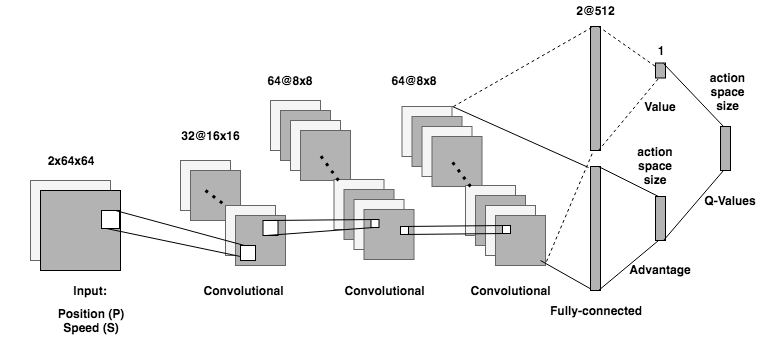
\includegraphics[width=0.8\textwidth]{images/CNN.png}
  \caption{The architecture of the Deep Neural Network.}
  \label{fig:CNN}
\end{center}
\end{figure}

The neural network is the same used in \cite{Wang2016}. The Figure \ref{fig:CNN} illustrates the Deep Neural Network. Every agent has its own Neural Network copy in order to allow it to learn its own local policy since every agent is trained independently by using IDQN.

\subsection{Framework}

We use OpenAI's baseline framework \cite{baselines} to implement our Dueling Prioritized DDQN. OpenAI Baselines is a set of high-quality implementations of reinforcement learning algorithms in Python which uses the library TensorFlow \cite{Abadi2016}. 

\section{Evaluation}

In this section we present an evaluation of IDQN as solution for multi-agent DRL for heterogeneous agents in traffic light control using the traffic simulator SUMO \cite{SUMO2012}. We run the test in the network layout show in Figure \ref{fig:simSetup}, which consists of three heterogeneous junctions. 

\begin{figure}
\begin{center}
  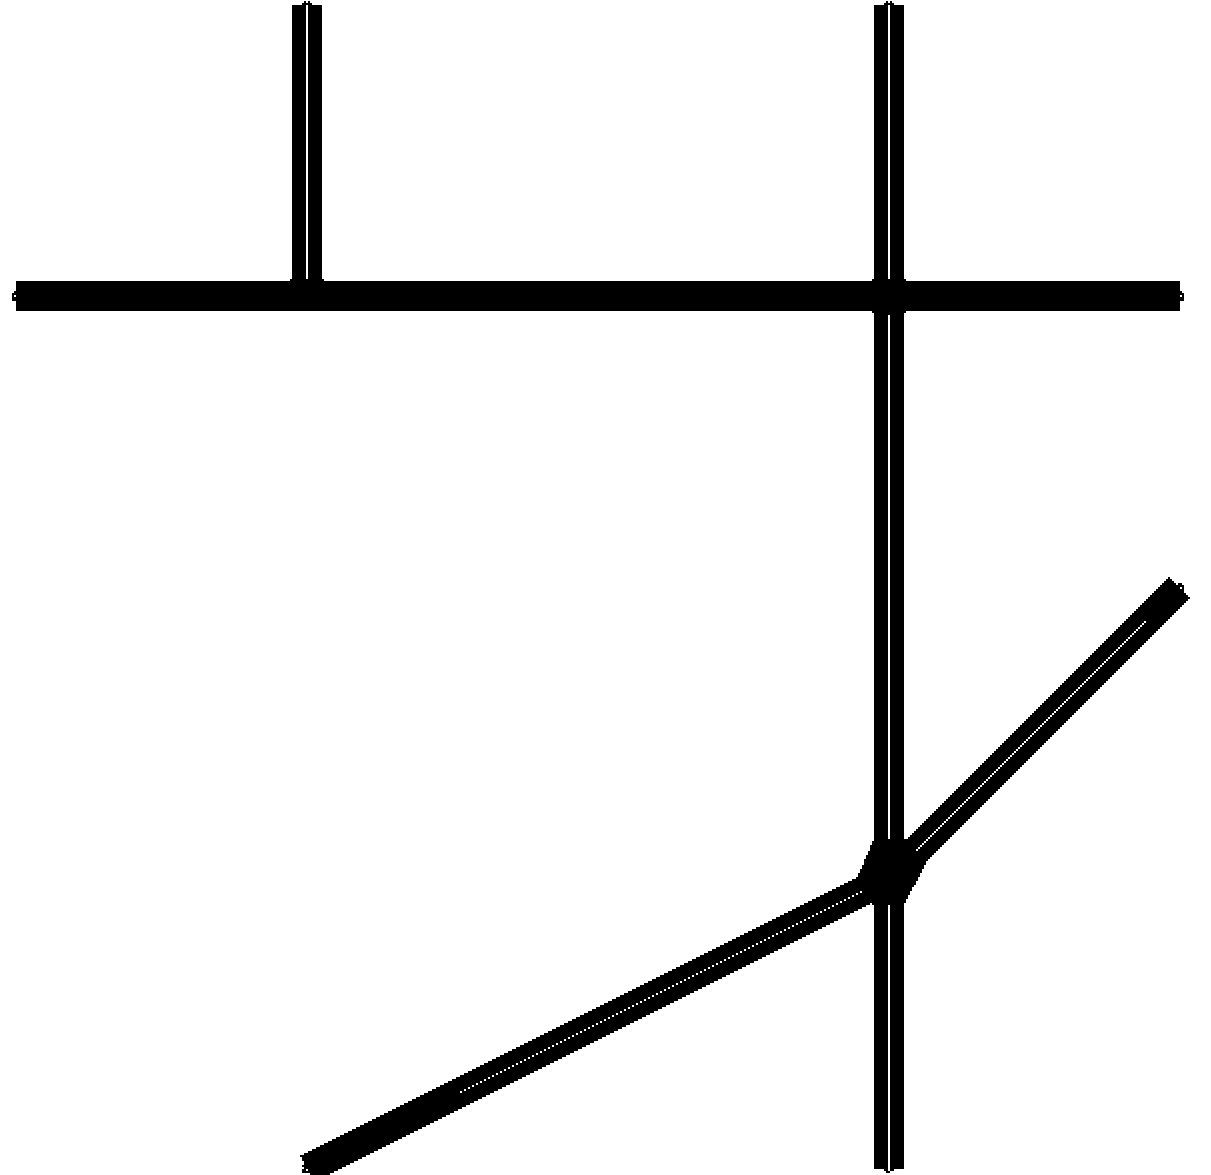
\includegraphics[width=0.15\textwidth]{images/MARL_env.png}
  \caption{Network Layout for Multi-Agent Experiments}
  \label{fig:simSetup}
\end{center}
\end{figure}

The table \ref{tab:MARLhyp} describes the hype-parameters used. Every episode corresponds to 1 hour of simulation time which is 3600 time steps, where every time step is 1 simulated second.

\begin{table}
\centering
\caption{Multi-agent evaluation hyper-parameters}
 \begin{tabularx}{\columnwidth}{X|X}
 \hline
 Parameter & Value \\ [0.5ex] 
 \hline
 \hline
 Episodes & 1000 \\
 Time steps & 3600000 \\
 Pre train time steps & 2500 \\
 Learning rate & 0.0004 \\
 Exploration $\epsilon$ & 1.0 $\rightarrow$ 0.01 \\
 Time steps from starting $\epsilon$ to ending $\epsilon$ & 360000 \\
 Target network update & 5000 \\
 Prioritization exponent $\alpha$ & 0.6 \\
 Prioritization importance sampling $\beta$ & 0.4 $\rightarrow$ 1.0 \\
 Discount factor $\gamma$ & 0.99 \\
 Replay Memory size M & 30000 \\
 Minibatch size B & 32 \\
 \hline
\end{tabularx}
\label{tab:MARLhyp}
\end{table}

We select two metrics that have been used in several DRL studies for UTC. Every metric is taken per episode. The metrics are the following:

\begin{itemize}
	\item \textbf{Cumulative Reward}. The reward \textit{r$_{t}$} taken on every time step \textit{t} is accumulated until the episode is finished.
	
	\item \textbf{Average Waiting Time}. It is is the sum of all \textit{W$_{t}$} divided by the number of time steps in the episode (N) as shown in Equation \ref{eq:AWT}. SUMO defines the waiting time for a vehicle as the time (in seconds) spent with a speed below 0.1 m/s since the last time it was faster than 0.1 m/s.
\begin{equation}\label{eq:AWT}
AWT = \frac{\sum^{t=1}_{N}{W_{t}}}{N}
\end{equation}
\end{itemize}

We evaluate the following techniques:

\begin{itemize}
\item \textbf{Fixed Time / Round Robin (FT)}. This is a predefined configuration for all the traffic lights where the duration and order of the phases is fixed and pre configured.

\item \textbf{IDQN without experience replay (ERM Disabled)}. It is a IDQN technique but the experience replay is disabled, therefore the agent cannot store experiences.

\item \textbf{IDQN with prioritized experience replay (PERM)}. It is a normal IDQN technique which uses the experience replay as recommended for DQN.

\item \textbf{IDQN with prioritized experience replay and fingerprint (PERM + FP)}. This is the proposed IDQN technique with the fingerprint to disambiguate the age of experience replays.

\item \textbf{IDQN with standard experience replay (ERM)}. This is IDQN with the standard experience replay, not with prioritized experience replay.
\end{itemize}

Every technique is tested in the following scenarios:

\begin{itemize}
\item \textbf{Low traffic load}. A scenario where the number of vehicles is reduced. It represents a normal flow where is not peek time. However, it is a good amount of cars to produce traffic jams if the traffic control is not good.
\item \textbf{High traffic load}. A scenario where the number of vehicles is overwhelming. It represents the traffic load in peek times. This scenario certainly will produced long queues and traffic jams even with good control. The idea is to verify if it is possible and how much can be reduced in such a overcrowded scenario.
\end{itemize}

\subsection{Experiments}

The Figure \ref{fig:LowHighIDQNExp} presents the results of the experiments executed in low and high traffic load respectively.

\begin{figure}[ht!]
    \centering
    \begin{subfigure}[b]{0.48\textwidth}
        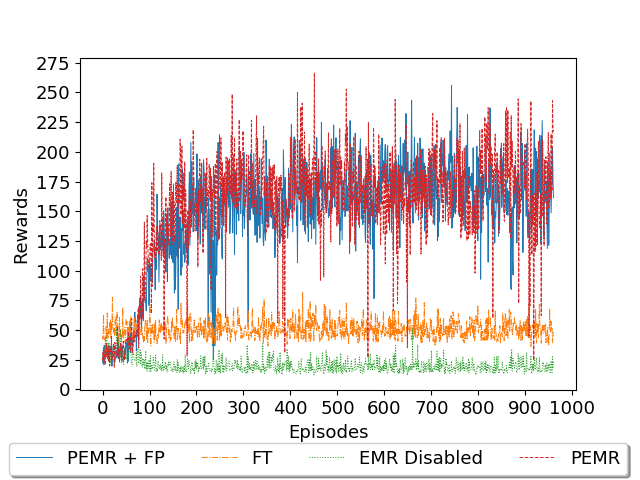
\includegraphics[width=\textwidth]{images/Low-Load-REW.png}
  		\caption{Low Traffic: Cumulative Rewards}
  		\label{fig:LowIDQNREW}
    \end{subfigure}
    \begin{subfigure}[b]{0.48\textwidth}
        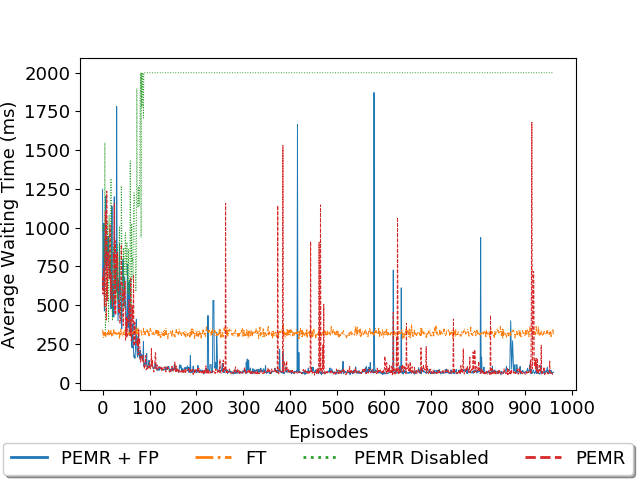
\includegraphics[width=\textwidth]{images/Low-Load-AWT.png}
  		\caption{Low Traffic: Average Waiting Time}
  		\label{fig:LowIDQNAWT}
    \end{subfigure}
     \begin{subfigure}[b]{0.48\textwidth}
        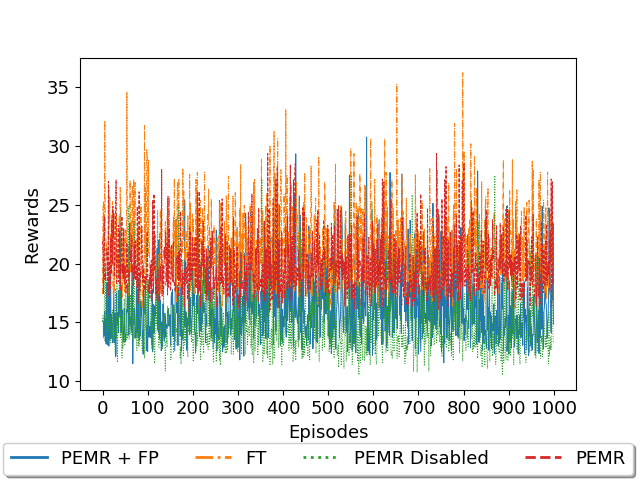
\includegraphics[width=\textwidth]{images/High-Load-REW.png}
  		\caption{High Traffic: Cumulative Rewards}
  		\label{fig:HighIDQNREW}
    \end{subfigure}
    \begin{subfigure}[b]{0.48\textwidth}
        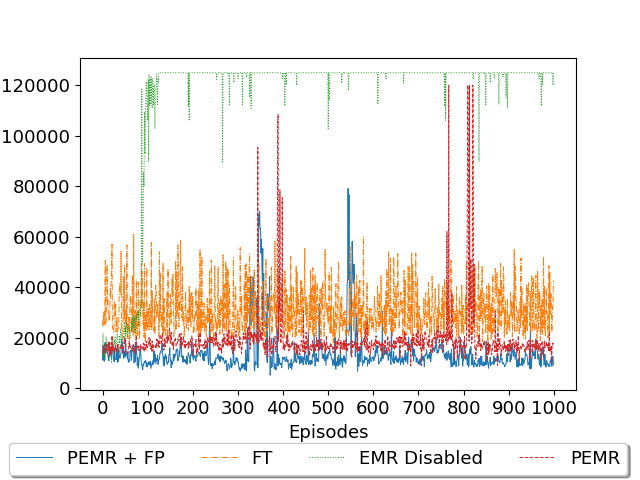
\includegraphics[width=\textwidth]{images/High-Load-AWT.png}
  		\caption{High Traffic: Average Waiting Time}
  		\label{fig:HighIDQNAWT}
    \end{subfigure}
    \caption{IDQN Experiments - Results per Episode}\label{fig:LowHighIDQNExp}
\end{figure}

%\begin{figure}
 %   \centering
  %  \begin{subfigure}[b]{0.48\textwidth}
   %     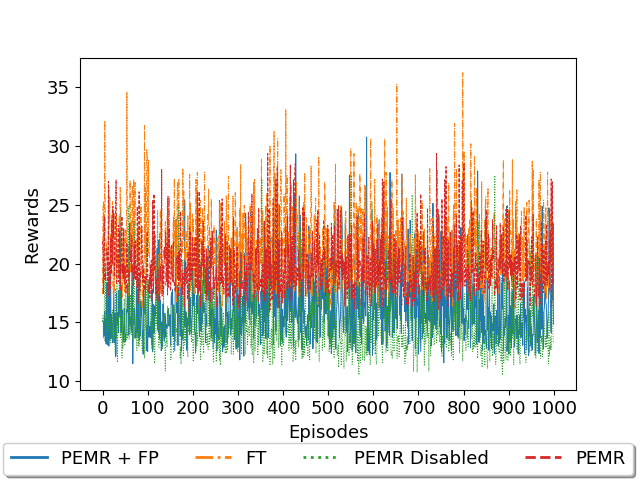
\includegraphics[width=\textwidth]{images/High-Load-REW.png}
  	%	\caption{Cumulative Rewards per Episode}
  	%	\label{fig:HighIDQNREW}
    %\end{subfigure}
    %\begin{subfigure}[b]{0.48\textwidth}
     %   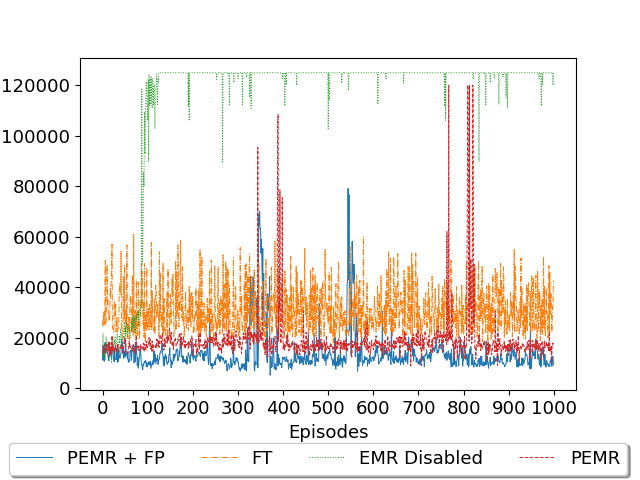
\includegraphics[width=\textwidth]{images/High-Load-AWT.png}
  		%\caption{Average Waiting Time per Episode}
  		%\label{fig:HighIDQNAWT}
    %\end{subfigure}
    %\caption{High Traffic IDQN Experiments}\label{fig:HighIDQNExp}
%\end{figure}

As can be seen from the Figure \ref{fig:LowIDQNREW}, \textit{FT} gets a constant reward range that varies extremely low around 50 due to it does not adjust its performance. Also, \textit{EMR Disabled} gets very bad rewards, even worse than the FT, and it never learns. Therefore, disabling the experience replay is not useful for our problem. Finally, we compare \textit{PERM} and \textit{PERM + FP}, which show identical performance getting 400$\%$ bigger rewards than \textit{FT}. They also learn very well in spite of the non-stationarity, increasing the rewards from around 25-100 in the exploration phase up to around 200-250 in the exploitation phase. They reach their optimal point at 300 episodes, where they get to keep a stable rewarding. Based on this similarity of results, we deduce that the fingerprint is not helping.

As illustrated in figure \ref{fig:HighIDQNREW}, \textit{FT} seems to make a good job in this scenario along with \textit{PERM}, both outperforms \textit{EMR Disabled} and \textit{PERM + FP} in around 25$\%$. It seems that the extra layer of the fingerprint reduces the performance of the technique under intense traffic loads. Moreover, none DRL technique gets to learn over the episodes. This can indicate that the agents needs more training for such a high load. 

The Figure \ref{fig:LowIDQNAWT} presents the waiting time for low traffic. \textit{FT} gets the same  behaviour than the rewards. In the case of \textit{EMR Disabled}, it  produces extremely high waiting times. Alike in rewards, \textit{PERM} and \textit{PERM + FP} get similar performance, with very low waiting times which are approximately 300$\%$ less than \textit{FT}. From these results we can also conclude that the fingerprinting is not helping. In high traffic load, the the results are similar. \textit{PERM + FP} outperform slightly \textit{PERM}. Alike the rewarding results, there is not learning across the training.

The unexpected performance of the fingerprint can be caused by:  

\begin{itemize}
\item \textbf{Not proper selection of fingerprint.} Fingerprint do not correlate enough with the true value of state-action pairs given the other agents' policies and/or it does not vary smoothly over training, which does not allow the model to generalise across experiences in which the other agents execute policies as they learn.
\item \textbf{Prioritized experience replay is good enough to deal with the non-stationarity.} Due to importance weights that allow to know what records are more valuable samples, which helps to disambiguate the age of the data.
\end{itemize}

We only verify the second hypothesis by executing a test with \textit{EMR}. The figure \ref{fig:ERMIDQNExp} shows this additional experiment which compares \textit{EMR} against \textit{PERM + FP}. As shown in Figure \ref{fig:ERMIDQNREW}, both techniques learn well, but \textit{PERM + FP} obtains higher rewards outperforming \textit{ERM} in around 45$\%$ in the highest point of \textit{PERM + FP}. Figure \ref{fig:ERMIDQNAWT} illustrates how they get a similar performance in waiting time, but \textit{EMR} is  more stable than \textit{PERM + FP} by not producing peeks. Regardless of the waiting time, we conclude the Prioritized Experience Replay helps to deal with the non-stationarity by getting bigger rewards, which indicates that \textit{PERM} has better performance than \textit{EMR}. The waiting time results are a direct result of the reward function, and \textit{PERM} is getting better results. It could be a correlation problem of the reward function if the waiting time is not decreasing proportionally to the rewards. These results prove that \textit{PERM} can be good enough to deal with the non-stationarity. However, \textit{PERM + FP} could improve by selecting a better fingerprint.

\begin{figure}[!htbp]
    \centering
    \begin{subfigure}[b]{0.48\textwidth}
        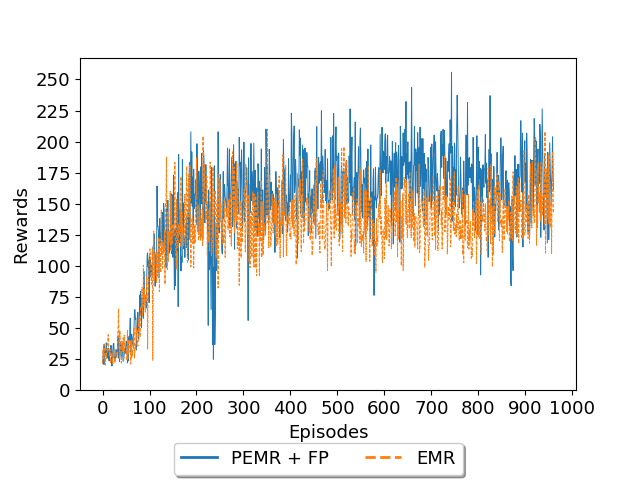
\includegraphics[width=\textwidth]{images/ERM-Low-Load-REW.png}
  		\caption{Cumulative Rewards per Episode}
  		\label{fig:ERMIDQNREW}
    \end{subfigure}
    \begin{subfigure}[b]{0.48\textwidth}
        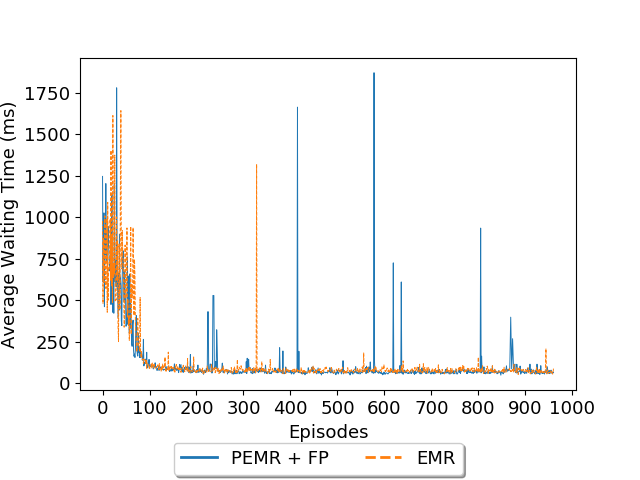
\includegraphics[width=\textwidth]{images/ERM-Low-Load-AWT.png}
  		\caption{Average Waiting Time per Episode}
  		\label{fig:ERMIDQNAWT}
    \end{subfigure}
    \caption{Low Traffic IDQN Experiments with Standard ERM}\label{fig:ERMIDQNExp}
\end{figure}

\section{Conclusion}

This paper presented IDQN as the only study which addresses heterogeneous multi-agent DRL in UTC. We implemented a IDQN by giving a Dueling Prioritized DDQN to each agent. We evaluated IDQN's performance with different configurations. We executed tests in two traffic conditions, i.e low and high traffic loads. Our experiments showed the IDQN is a suitable techniques for heterogeneous multi-agent UTC environments which can deal with the non-stationarity. The best results were obtained in the low traffic load. The high traffic load seems to need longer training time. We demonstrated that IDQN outperforms the baseline, and that the experience replay is mandatory to learn efficiently. Nonetheless, the fingerprint we chose do not enhance the normal prioritized experience replay.

Finally, PERM needs further investigation to find out better fingerprints. Also, the integration of the fingerprint as an additional matrix can be studied to verify if it is the best approach in a RL system fed with image-like states.

% --- BIBLIOGRAPHY
\bibliographystyle{splncs03}
\bibliography{aics-sample} 

\end{document}
